% !TEX TS-program = pdflatexmk
\documentclass[12pt]{article}

% Layout.
\usepackage[top=1in, bottom=0.75in, left=1in, right=1in, headheight=1in, headsep=6pt]{geometry}

% Fonts.
\usepackage{mathptmx}
\usepackage[scaled=0.86]{helvet}
\renewcommand{\emph}[1]{\textsf{\textbf{#1}}}
\newcommand{\ans}[1][1in]{\rule{#1}{.5pt}}

\usepackage[parfill]{parskip}

% Misc packages.
\usepackage{amsmath,amssymb,latexsym}
\usepackage{graphicx,hyperref}
\usepackage{array}
\usepackage{xcolor}
\usepackage{multicol,tikz}
\usetikzlibrary{calc, positioning}
\usepackage{tabularx,colortbl,booktabs,xparse}
\usepackage{enumitem}

% Rotation: \rot[<angle>][<width>]{<stuff>}
\NewDocumentCommand{\rot}{O{45} O{1em} m}{\makebox[#2][l]{\rotatebox{#1}{#3}}}%

\usepackage{fancyhdr}
\pagestyle{fancy}
\lhead{\large\sf\textbf{MATH F113X: Graph Theory}}
\chead{\large\sf\textbf{lecture notes}}
\rhead{\large\sf\textbf{Intro}}

\begin{document}
Goal: See \emph{why} we might model a situation with a graph, and learn some vocabulary.

\begin{enumerate}
\item  %Consider these situations / contexts:
%
%\begin{enumerate}
%\item The road system connecting some towns in Alaska.
%\item The streets in a neighborhood that a snowplow has to clear after a storm.
%\item A group of people, and who is friends with whom.
%\item The classes offered at this university, and the students that take them.
%\end{enumerate}


\vspace{.1in}

%\begin{center}
%\fbox{
%\begin{tabular}{r p{3.3in}}
\emph{vertex} (plural: \emph{vertices}):  %one of the things, drawn as a dot or a labeled box\\[6pt]

\emph{edge:}  %a connection between two of them, drawn as a line or curve
%\end{tabular}

%========================================================





\vspace{.1in}


{\renewcommand{\arraystretch}{2.4}
\begin{tabularx}{\linewidth}{|p{3.5in}|X|X|}
\hline
\emph{situation} & \emph{vertices are\ldots} & \emph{edges are\ldots} \\ \hline
The road system connecting some towns in Alaska. & & \\ \hline
The streets in a neighborhood that a snowplow has to clear after a storm. & & \\ \hline
A group of people, and who is friends with whom. & & \\ \hline
Classes offered at this university, and the students that take them. & & \\[.42in] \hline
\end{tabularx}
}

\vspace{.15in}

%========================================================
\item We have information about five people and who is friends with whom. Draw a graph. %What are the vertices? What are the edges?

%\medskip

\begin{minipage}[t]{0.3\linewidth}
\vspace{0pt}
\begin{tabular}{l|l}
\emph{person} & \emph{friends with} \\ \hline
Rosa & Sam, Tavi \\
Sam & Rosa, Tavi, Uma \\
Tavi & Rosa, Sam \\
Uma & Sam, Wes \\
Wes & Uma \\
\end{tabular}
\end{minipage}

\bigskip
%\hfill
%\begin{minipage}[t]{0.66\linewidth}
%\vspace{0pt}
%\rule{0pt}{2.05in}
%\end{minipage}



%========================================================
\item  Are these all the same graph? How can we tell? (What does ``same'' mean?)

\begin{center}
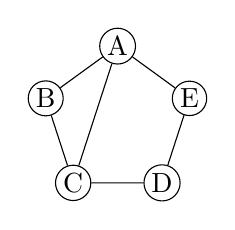
\begin{tikzpicture}[scale=.6, vtx/.style={draw, circle, inner sep = 1 pt}, baseline=(current bounding box.north)]
\node[vtx] (A) at (90:1.6) {A};
\node[vtx] (B) at (162:1.6) {B};
\node[vtx] (C) at (234:1.6) {C};
\node[vtx] (D) at (306:1.6) {D};
\node[vtx] (E) at (18:1.6) {E};
\draw (A) -- (B) -- (C) -- (D) -- (E) -- (A);
\draw (A) -- (C);
\end{tikzpicture}
%\hspace{1in}
\hfill
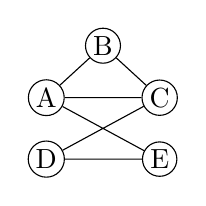
\begin{tikzpicture}[scale=.6, vtx/.style={draw, circle, inner sep = 1 pt}, baseline=(current bounding box.north)]
\node[vtx] (A) at (0,0) {A};
\node[vtx] (C) at (2.4,0) {C};
\node[vtx] (B) at (1.2,1.1) {B};
\node[vtx] (E) at  (2.4,-1.3) {E};
\node[vtx] (D) at (0,-1.3) {D};
\draw (A) -- (B) -- (C) -- (A);
\draw (A) -- (E) -- (D) -- (C);
\end{tikzpicture}
\hfill
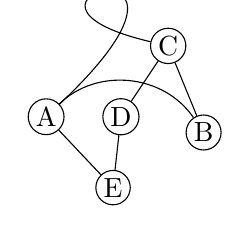
\begin{tikzpicture}[scale=.5, vtx/.style={draw, circle, inner sep = 1 pt}, baseline=(current bounding box.north)]
\node[vtx] (A) at (0,0.3) {A};
\node[vtx] (C) at (3.1,2.1) {C};
\node[vtx] (D) at (1.9,0.3) {D};
\node[vtx] (E) at (1.7,-1.5) {E};
\node[vtx] (B) at (4.0,-0.1) {B};
\draw (A) to [bend left = 50] (B);
\draw[-, overlay] (A) .. controls ($(C)+(2,3)$) and ($(A)+(-2,3)$) .. (C);
\draw (C) -- (D);
\draw (D) -- (E);
\draw (A) -- (E);
\draw (C) -- (B);
\end{tikzpicture}
\hfill
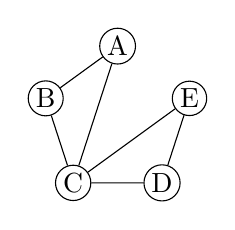
\begin{tikzpicture}[scale=.6, vtx/.style={draw, circle, inner sep = 1 pt}, baseline=(current bounding box.north)]
\node[vtx] (A) at (90:1.6) {A};
\node[vtx] (B) at (162:1.6) {B};
\node[vtx] (C) at (234:1.6) {C};
\node[vtx] (D) at (306:1.6) {D};
\node[vtx] (E) at (18:1.6) {E};
\draw (A) -- (B) -- (C) -- (D) -- (E) -- (C);
\draw (A) -- (C);
\end{tikzpicture}
\end{center}

%Why does this matter?
%
%\vspace{1.3in}

\newpage

%========================================================
\item Below is a neighborhood: each vertex is an intersection, each edge is a street. How busy is each intersection? %The \emph{degree} of a vertex is the number of edge-ends meeting it. A \emph{loop} --- an edge from a vertex back to itself --- counts \emph{twice}.

{\bf Degree}  

{\bf Loop degree}   

\begin{center}
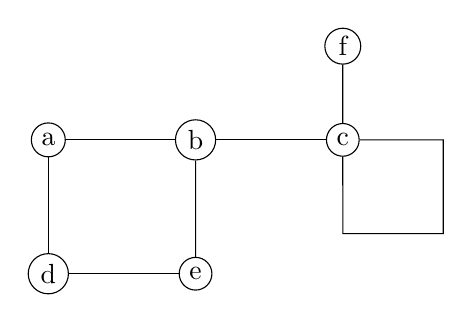
\begin{tikzpicture}[scale=.85, vtx/.style={draw, circle, inner sep = 2 pt}]
\node[vtx] (a) at (0,2) {a};
\node[vtx] (b) at (2.2,2) {b};
\node[vtx] (c) at (4.4,2) {c};
\node[vtx] (d) at (0,0) {d};
\node[vtx] (e) at (2.2,0) {e};
\node[vtx] (f) at (4.4,3.4) {f};
\draw (a) -- (b) -- (c);
\draw (a) -- (d);
\draw (b) -- (e);
\draw (d) -- (e);
\draw (c) -- (f);
\draw (c) -- (5.9,2) -- (5.9,0.6) -- (4.4,0.6) -- (c);
\end{tikzpicture}
\end{center}

degree of $a$: \ans[.5in] \quad $b$: \ans[.5in] \quad $c$: \ans[.5in] \quad $d$: \ans[.5in] \quad $e$: \ans[.5in] \quad $f$: \ans[.5in]

%\newpage

%========================================================
\item Below is a road network: each vertex is a town, each edge is a road.

\begin{center}
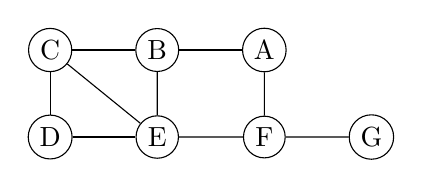
\begin{tikzpicture}[scale=.85, vtx/.style={draw, circle, inner sep = 2 pt}]
\node[vtx] (C) at (0,1.3) {C};
\node[vtx] (B) at (1.6,1.3) {B};
\node[vtx] (A) at (3.2,1.3) {A};
\node[vtx] (D) at (0,0) {D};
\node[vtx] (E) at (1.6,0) {E};
\node[vtx] (F) at (3.2,0) {F};
\node[vtx] (G) at (4.8,0) {G};
\draw (A) -- (B) -- (C);
\draw (C) -- (E) -- (F) -- (G);
\draw (A) -- (F);
\draw (B) -- (E);
\draw (C) -- (D) -- (E);
\end{tikzpicture}
\end{center}

\begin{enumerate}
\item {Can I get from here to there?}

\emph{path:}

\bigskip

Find a path from $D$ to $G$: \ans[2.5in]

\vspace{.15in}

\item {Can I leave home and get back?}

\emph{circuit: } %is a path that starts and ends at the same vertex.

\bigskip

Find a circuit starting at $E$: \ans[2.5in]

\vspace{.15in}

\item {Is everything reachable at all?}

\emph{connected:} %if there is a path between every pair of vertices.

\bigskip

Which graphs are connected? %\ans[.7in]

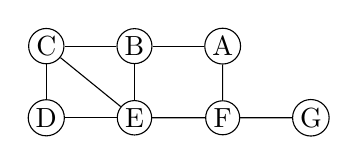
\begin{tikzpicture}[scale=.7, vtx/.style={draw, circle, inner sep = 1 pt}]
\node[vtx] (C) at (0,1.3) {C};
\node[vtx] (B) at (1.6,1.3) {B};
\node[vtx] (A) at (3.2,1.3) {A};
\node[vtx] (D) at (0,0) {D};
\node[vtx] (E) at (1.6,0) {E};
\node[vtx] (F) at (3.2,0) {F};
\node[vtx] (G) at (4.8,0) {G};
\draw (A) -- (B) -- (C);
\draw (C) -- (E) -- (F) -- (G);
\draw (A) -- (F);
\draw (B) -- (E);
\draw (C) -- (D) -- (E);
\end{tikzpicture}
\hfill
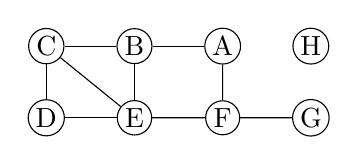
\begin{tikzpicture}[scale=.7, vtx/.style={draw, circle, inner sep = 1 pt}]
\node[vtx] (C) at (0,1.3) {C};
\node[vtx] (B) at (1.6,1.3) {B};
\node[vtx] (A) at (3.2,1.3) {A};
\node[vtx] (D) at (0,0) {D};
\node[vtx] (E) at (1.6,0) {E};
\node[vtx] (F) at (3.2,0) {F};
\node[vtx] (G) at (4.8,0) {G};
\node[vtx, ] (H)at (4.8,1.3){H};
\draw (A) -- (B) -- (C);
\draw (C) -- (E) -- (F) -- (G);
\draw (A) -- (F);
\draw (B) -- (E);
\draw (C) -- (D) -- (E);
\end{tikzpicture}
\hfill
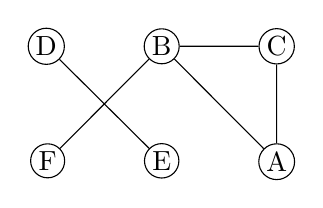
\begin{tikzpicture}[scale=.7, vtx/.style={draw, circle, inner sep = 1 pt}]
%\node[vtx] (C) at (0,1.3) {C};
%\node[vtx] (B) at (1.6,1.3) {B};
%\node[vtx] (A) at (3.2,1.3) {A};
%\node[vtx] (D) at (0,0) {D};
%\node[vtx] (E) at (1.6,0) {E};
%\node[vtx] (F) at (3.2,0) {F};
%\node[vtx] (G) at (4.8,0) {G};
%\node[vtx, ] (H)at (4.8,1.3){H};
%\draw (A) -- (B) -- (C);
%\draw (C) -- (E) -- (F) -- (G);
%\draw (A) -- (F);
%\draw (B) -- (E);
%\draw (C) -- (D) -- (E);

\node[vtx] (C) at (0,0){C};
\node[vtx, left = of C] (B){B};
\node[vtx,left = of B] (D){D};
\node[vtx,below = of C] (A){A};
\node[vtx, below = of B] (E){E};
\node[vtx,left = of E] (F){F};
\draw (F) -- (B) -- (A) -- (C) -- (B);
\draw (D) -- (E);
\end{tikzpicture}


\end{enumerate}

%\vspace{.3in}

%========================================================
%\item \emph{Where we are going.}
%
%\bigskip
%
%{\renewcommand{\arraystretch}{2.4}
%\begin{tabularx}{\linewidth}{|p{2.4in}|X|}
%\hline
%\emph{the question} & \emph{a situation where you would ask it} \\ \hline
%What is the cheapest way to connect everything? & \\ \hline
%Is there a route that covers every \emph{edge} and returns home? & \\ \hline
%Is there a route that visits every \emph{vertex} and returns home? & \\ \hline
%\end{tabularx}
%}
%
%\vspace{.5in}
%
%Which of the last two is harder? Why?
%
%\vfill

\end{enumerate}
\end{document}
